% Copyright (c) 2026 Jonathan Yantis. SPDX-License-Identifier: CC-BY-4.0
\documentclass[10pt,letterpaper]{article}
\usepackage[T1]{fontenc}\usepackage{lmodern}
\usepackage[margin=.73in]{geometry}
\usepackage{amsmath,booktabs,graphicx,array,microtype,natbib,fancyhdr}
\usepackage[colorlinks=true,urlcolor=blue,citecolor=blue,linkcolor=blue]{hyperref}
\hypersetup{pdftitle={Paired Clock Time Transfer from Starlink over Wi-Fi},pdfauthor={Jonathan Yantis},pdfsubject={Author-review draft: paired local/AP clocks, causal filtering and calibrated GNSS-input phase comparisons}}
\setlength{\parskip}{4pt}\setlength{\parindent}{0pt}
\pagestyle{fancy}\fancyhf{}\fancyhead[L]{\small Starlink paired-clock experiments}
\fancyhead[R]{\small Author-review draft}\fancyfoot[C]{\thepage}
\setlength{\headheight}{14pt}
\newcommand{\us}{\ensuremath{\,\mu\mathrm{s}}}
\newif\ifPrimaryResultsReady
\PrimaryResultsReadytrue
\title{Paired Clock Time Transfer from Starlink over Wi-Fi:\\Causal Filtering, Drift, and GNSS-Shadow Validation}
\author{Jonathan Yantis}
\date{3 November 2026 (UTC) --- Research preprint for author review}
\begin{document}
\maketitle\thispagestyle{fancy}
\begin{abstract}
We test whether ordinary Wi-Fi beacon timing adds useful clock information to
Starlink terminal NTP when AP UTC alignment and discipline are unknown.
AP-assisted estimates are compared with an AP-free NTP/local baseline and
matched controls. GNSS-shadow PPS supplies each method's fixed prior phase
base and a validation witness, never a frequency correction. Two SL027 windows
each allocate 900 seconds to training and 900 to future evaluation, with filter
parameters locked using earlier data. Continuous estimates retain a 60-second
source lease; longer frozen forecasts are research holdover.
On all 900 future PPS per window, the nominated robust AP model reduces
prior-phase-corrected RMS from the AP-free control's 37.180 to 19.226\us\ and
from 35.662 to 8.240\us. The first gain reduces bias while slightly worsening
centered scatter; the second reduces both. Ordinary AP fits and servos have
mixed outcomes. Raw phase RMS remains above 200\us; earlier failures and
incomplete histories remain separate. AP information can differ from the local
clock, but constant-rate cancellation does not remove AP wander, NTP bias or
asymmetry. These externally calibrated PPS-input comparisons do not establish
portable GNSS-free UTC accuracy or measured output.
\end{abstract}

\section{Question, clock domains and prior work}
Starlink describes its terminal NTP as GPS-based and best-effort, with no
accuracy guarantee \citep{starlink}. The access point broadcasts TSF time,
but we have not measured its discipline relative to the terminal.
Terminal, AP, client MAC, local timer and capture counter form observable
clock domains; their physical dependencies remain unresolved.

Deployment requires an existing dish/AP and a client exposing receive-event
timestamps. Our client is an ESP32-S3 W12; ordinary phone/laptop APIs need not
expose equivalent information. Qualification adds GNSS hardware. The measured
phase base is not portable across clients, paths, boots or models.

The motivating beacon record gave 0.409\us\ causal relative RMS over 600 seconds,
with one missing raw record and a failed no-gap gate. A separate shadow-PPS
observation showed about 6.447 ppm AP gain: small relative residuals do not
establish GPS alignment. Espressif specifies microsecond timestamp units and
sleep conditions, not RF endpoint bias or UTC accuracy \citep{espheader}.

Delay filtering and clock discipline are established \citep{rfc5905,chrony}.
Averaging trades network-jitter suppression against oscillator-wander tracking
\citep{ntpdiscipline}. Two-timescale designs still cannot partition clock/network
noise without ancillary information \citep{levine2016}; even ideal affine clocks
have offset/directional-delay ambiguities \citep{freris2011}. This is a paired
experiment, not a first-use, optimal-filter or accuracy-ranking claim.

\section{Causal observations and paired models}
\subsection{NTP and the two clock coordinates}
The client timestamps immediately before connected UDP \texttt{send} and after
\texttt{recv} returns, giving local $T_1,T_4$; NTP supplies server receive and
transmit $T_2,T_3$. The conventional estimates are \citep{rfc5905}
\begin{equation}
 \theta_i=\tfrac12[(T_2-T_1)+(T_3-T_4)],\qquad
 \delta_i=(T_4-T_1)-(T_3-T_2).
\end{equation}
These software endpoints retain stack, scheduling and directional-transfer
bias; subtracting server residence does not identify it. The requests address
the local terminal service, not satellite RF timing. Admission checks protocol,
transaction, context and timing bounds. Eight requests about one second apart
per 16 seconds yield one lowest-RTT observation per complete burst, newer replies
winning ties. Refused/incomplete bursts are retained. Runtime
\texttt{MIN\_RTT8} instead chooses the lowest-delay valid anchor from the latest
eight accepted exchanges; neither policy implements full NTP discipline.

Let $L$ denote separately read local-timer microseconds, $A$ AP TSF microseconds,
$q$ raw 80 MHz capture ticks and $U$ the NTP UTC coordinate. A prior affine map
connects $q$ to $L$. Separate prior maps connect $q$ to the client MAC receive
counter and then to AP beacons. For an NTP endpoint, the AP map must commit
before the independent local-map read begins, and that read must precede the
endpoint. The certified map is inverted to place the endpoint in $q$, then
projected into $A$. Exact split midpoint coordinates retain half-microsecond
parity; integer UTC/AP origins avoid subtracting large floating-point epochs.
All input replies must already have arrived before model publication.

The AP/local pair fits the \emph{same AP-mappable burst minima} with identical
weights. For coordinate $X\in\{L,A\}$, the matched affine model is
\begin{equation}
 \begin{gathered}
 \widehat U_X(X)=U_0+a_X+k_X(X-X_0),\\
 (a_X,k_X)=\arg\min_{a,k}\sum_i w_i[U_i-U_0-a-k(X_i-X_0)]^2,
 \qquad w_i=\max(\delta_i,1\us)^{-2}.
 \end{gathered}
\end{equation}
Here $k_X$ is a dimensionless UTC-microseconds/coordinate-microseconds ratio.
Inverse-squared RTT is a declared heuristic, not a measured inverse variance.
A separate all-NTP/local control retains minima whose AP endpoint is unavailable.
The primary system comparison uses the nominated robust AP model against this
AP-free NTP/local 900-second WLS baseline, on identical future witnesses and
with each estimator's own prior fixed phase base. Weighting and coordinate can
both differ; any gain is not uniquely an AP-oscillator effect. The shared-Huber
local model is a secondary mechanism control: its AP-derived weights mean that
it is not AP-free. Where AP-mappable input populations differ, their selection
effect is also reported separately.

\subsection{What the AP can add}
If $A=\alpha+\beta L$ exactly over training and prediction, matched affine
fits in $A$ and $L$ are algebraically equivalent. Cancelling constant AP drift
adds no information; potential value comes from non-affine stability/noise.
The exact dual-rate relation is
\begin{equation}
 \frac{dU}{dL}=\frac{dU}{dA}\frac{dA}{dL}.
\end{equation}
Slow NTP/AP calibration estimates $dU/dA$; frequent beacons/maps track $dA/dL$.
A steadier AP may attenuate local-rate changes, but AP wander leaks until the
slow loop responds. Exact AP/local subtraction returns the local coordinate;
finite-bandwidth smoothing cannot guarantee zero AP inheritance. Client MAC
independence from AP discipline and the RF timestamp endpoint remain uncalibrated.

\subsection{Admission, availability and phase scoring}
History is bounded to 900 seconds and 128 minima. At least eight points spanning
60 seconds are needed. A prior \emph{unweighted} local OLS model gates a new
minimum. For its earlier residuals $r_k$, set
$s=1.4826\operatorname{median}|r_k-\operatorname{median}(r)|$; the threshold is
\begin{equation}
 G_i=\max(50\us,6s)+\tfrac12\max(0,\delta_i-\delta_{\min,\mathrm{prior}}).
\end{equation}
The final fit uses the declared RTT weights. Three consecutive rejected minima
clear history and require reacquisition. The gate can reject a true clock step;
smooth contamination and early points admitted before initialization can pass.
A separate 50\us\ beacon-prediction innovation withdraws AP source context. It
does not identify the cause or detect every step or smooth wander.

GNSS PPS is captured in $q$ and projected using a snapshot committed strictly
before the physical edge, with a 250 ms bridge lease and a fix known before it.
The raw witness is retained even if a map is unavailable. AP unavailability
means \emph{unknown}, never a substituted local coordinate or zero error. A
network-generation change resets models; an AP-population change resets paired
AP-dependent history. Capture-map epochs cannot identify AP clock corrections.

For each window, the AP-available members of the last 16 qualified pre-cutoff
PPS form one identical calibration identity set, with at least eight required.
Each method has its own fixed base $B_X$. Frozen models retrodict these earlier
PPS with their sealed final fit; continuous methods use only their actual prior
predictions at those edges. Subsequent error is
\begin{equation}
 e_j=\operatorname{phase}_{1\mathrm{s}}[\widehat U_X(X_j)]-B_X.
\end{equation}
No GNSS frequency, future error or validation mean trains a correction. Raw
phase is reported separately: an installation without the measured GNSS base
does not inherit phase-corrected RMS. Future recentering/detrending would be a
different metric and never changes the primary score. All future tails remain.
Modulo-one-second phase cannot itself detect an integer
UTC-second error. PPS association, receiver/wiring delay, RF endpoint bias and
electrical output uncertainty are not independently calibrated.

\section{Protocol and locked offline filter experiment}
Two SL027 windows, R1--R2, use one image/boot and fixed request cadence.
Wi-Fi power saving and automatic light sleep are disabled.
At least 300 seconds of full-logging warmup precede the first 1800-second window.
Each resets paired fitting, trains a native model for 900 seconds, then retains
900 future PPS. Frozen coefficients, inputs and phase bases are sealed before
future inspection. Eight-second expiry audits omit complete beacon/map history;
30 seconds of recorded reprime follow. Missing history remains unknown. A
pre-access collector startup failure supplies no timing observations. Frozen
source age beyond 60 seconds is research holdover, not continuous service.

Filters/nominations were developed on historical SL025 P1 and locked before
P2/P3 heldout errors. Exact estimator code and parameters carry into both fresh
windows. After R1, the author reduced the original three-window plan to two
before R2 freeze/future scoring; R3 is not acquired, not a failed/missing trial. Plan
and amendment remain recorded; no filter is retuned or selected from SL027.

The semantic adapter excludes only isolated same-context refused AP maps from
the method view. They supply no point or renewed lease. Explicit reset/new-epoch
barriers and every raw/native-invalid record remain audited. An unfenced reset
bars a verified adapted comparison; no unavailable map is invented.
All declared candidates remain in validation:
\begin{itemize}\setlength{\itemsep}{0pt}
\item RTT-weighted affine fits over trailing 300 or 900 seconds, in matched
local/AP coordinates, plus a separate all-NTP/local control.
\item One robust 900-second pair: initial RTT WLS followed by five fixed Huber
reweighting iterations, $c=1.5$, with residual scale
$\max(10\us,1.4826\operatorname{MAD})$. AP-derived factors
$\min(1,1.5s/|r_i|)$ multiply RTT weights and are shared exactly with the local
fit. This is \emph{AP-assisted residual weighting}, not NTP-only filtering. Every
retained point has positive weight; no hand-picked point is deleted.
\item Two phase-continuous local/AP servo pairs, with 60 or 180-second phase
time constants, 300-second frequency averaging and a 10 ppm phase-slew cap.
\end{itemize}
Targets publish only after completed bursts at a subsequent committed map
with the prior AP certificate. Continuous source age uses the latest admitted
reply actually retained by that target; the 900-second history never extends
the 60-second lease.

Servos integrate split UTC in $q$ with $dU/dq=(dU/dX)(dX/dq)$, preserving phase
at updates. They average target rate over 300 seconds and add a 10 ppm-capped
phase correction $e/(10^6\tau)$, where $e$ is microseconds and $\tau=60$ or 180
seconds. Three target disagreements above 500\us\ withdraw/reacquire. AP absence
still withholds qualification. Software continuity is not physical output;
computation/publication worst-case latency is unmeasured. Huber AP900 and AP
servo60 were nominated from P1; the latter was not a development benefit.
Synthetic step/spike/continuity tests are distinct from field accuracy evidence.

\subsection{Client repairs and availability cohorts}
SL027 changes acquisition reliability, not these estimators. Four published
bridge slots plus one staging slot place coefficient copies before the
availability latch; only successful commits train/increment serials. Refusals
retain the prior model under its unchanged 250 ms lease. Each scheduled 100 ms
update allows one bounded fresh-read retry, never across a counter/source fault.
Integer continuity arithmetic preserves the 1000\us\ fence. A fresh counter
sample after each PPS dequeue repairs the newer-queued-edge/older-current race.
Reset/refusal telemetry distinguishes withdrawal from retained history.

SL026 qualification retains 600 physical/AP and 588 common projections, with
51 AP refusals and zero replay mismatches/new fault increments. Its 98.0\%
availability fails the 98.1\% gate. Relative to the declared historical 344/1799
baseline, the descriptive unavailable-fraction reduction is 89.54\%, not a
population failure bound. The author accepted that availability to proceed;
this neither passes the old gate nor qualifies the distinct SL027 image/boot.
No additional 600-second qualification precedes the new cohort.

\section{Measured comparisons and retained coverage}
The tables retain native failures and use the same physical PPS for each
local/AP comparison. Signed mean, population-centered standard deviation, RMS,
nearest-rank absolute P99 and maximum describe fixed-base PPS agreement. RMS is
$\sqrt{\mu^2+\sigma^2}$; it does not become an uncertainty bound because many
correlated PPS were collected. A descriptive future fit
$e_j=c+d\tau_j+\eta_j$ reports drift $d$ in microseconds per local second (ppm)
and detrended RMS. Neither $c$ nor $d$ corrects the accuracy scores
\citep{riley}.
A replayed window remains valid regardless of RMS; unavailable/unverified
states are separate quality classifications. Large future errors are never
discarded to satisfy a timing target.

\ifPrimaryResultsReady
% Generated by hybrid/analyze.py; CC BY 4.0 Jonathan Yantis.
% Generated by hybrid/analyze.py; CC BY 4.0 Jonathan Yantis.

\begin{table}[t]\centering\small
\caption{Prior-phase-corrected errors against shadow PPS in $\mu$s. NTP-only WLS and nominated robust AP hybrid use identical scored witnesses; ordinary AP WLS and the servo retain their declared paired populations. Each method uses its own fixed phase base on the same prior PPS subset, with no validation recentering or detrending.}
\label{tab:hybrid-accuracy}\begin{tabular}{llrrrrrr}\toprule
Run & Method & $n$ & Mean & Scatter & RMS & Abs. P99 & Max. abs. \\ \midrule
R1 & NTP-only WLS & 900 & -34.01 & 15.02 & 37.18 & 67.33 & 67.66 \\
R1 & Robust AP & 900 & 11.44 & 15.45 & 19.23 & 43.08 & 43.85 \\
R1 & AP WLS & 900 & -41.55 & 17.02 & 44.90 & 79.80 & 80.73 \\
R1 & AP servo 60 & 900 & -47.04 & 16.26 & 49.77 & 75.61 & 75.66 \\
R2 & NTP-only WLS & 900 & -32.61 & 14.43 & 35.66 & 54.77 & 55.21 \\
R2 & Robust AP & 900 & -4.79 & 6.70 & 8.24 & 20.07 & 20.24 \\
R2 & AP WLS & 900 & -17.70 & 12.04 & 21.40 & 40.78 & 40.93 \\
R2 & AP servo 60 & 900 & -2.22 & 8.97 & 9.24 & 19.77 & 20.09 \\
\bottomrule\end{tabular}

\end{table}

% Generated by hybrid/analyze.py; CC BY 4.0 Jonathan Yantis.

\begin{table}[t]\centering\small
\caption{Continuously updated offline methods, fixed own prior phase bases. Each cell is matched local/AP RMS in $\mu$s on the AP-common population. All primary runs use the locked candidates unchanged; historical exploratory P1 remains in the selected data. Huber weights are AP-derived and shared, so its local branch is also AP-assisted. No validation winner is selected.}
\label{tab:hybrid-filters}\begin{tabular}{lrr}\toprule
Method & R1 & R2 \\ \midrule
WLS 300 s & 82.08/82.74 & 61.16/60.94 \\
WLS 900 s & 37.18/44.90 & 33.91/21.40 \\
Shared-AP Huber 900 s & 24.46/19.23 & 20.40/8.24 \\
Continuous servo 60 s & 38.36/49.77 & 22.13/9.24 \\
Continuous servo 180 s & 40.82/56.79 & 14.91/8.51 \\
\midrule
All-NTP WLS 300 s & 82.08 & 61.82 \\
All-NTP WLS 900 s & 37.18 & 35.66 \\
Original MIN8 & 473.63 & 174.22 \\
\bottomrule\end{tabular}
\par\smallskip Single values use all-NTP inputs, scored on the same AP-common PPS subset.

\end{table}

% Generated by hybrid/analyze.py; CC BY 4.0 Jonathan Yantis.

\begin{table}[t]\centering\small
\caption{Training residual scatter includes NTP source, path, client endpoints and coordinate effects. It cannot isolate source-only jitter. Minima refer to the canonical frozen fit, before Huber downweighting.}
\label{tab:hybrid-jitter}\begin{tabular}{lrrrr}\toprule
Run & Accepted NTP (ms) & Local minima ($\mu$s) & AP minima ($\mu$s) & Gate rejects \\ \midrule
R1 & 3.897 & 217.11 & 217.38 & 0 \\
R2 & 4.556 & 102.74 & 102.97 & 0 \\
\bottomrule\end{tabular}
\end{table}

% Generated by hybrid/analyze.py; CC BY 4.0 Jonathan Yantis.

\begin{table}[t]\centering\small
\caption{Frozen forecasts after 900 s training: PPS-relative errors after the fixed prior phase base. All 900 future opportunities remain in each run. Beyond true source age 60 s these are research holdover, not qualified UTC service.}
\label{tab:hybrid-frozen}\begin{tabular}{lrrrrr}\toprule
Run & Known/900 & AP RMS & Local RMS & Fresh $n$ & Fresh AP/local RMS \\ \midrule
R1 & 900/900 & 35.168 & 65.843 & 44 & 1.977/2.923 \\
R2 & 900/900 & 31.777 & 50.824 & 58 & 2.146/3.999 \\
\bottomrule\end{tabular}
\par\smallskip All RMS entries are in $\mu$s; fresh means true source age $<60$ s.

\end{table}


\begin{figure}[tb]\centering
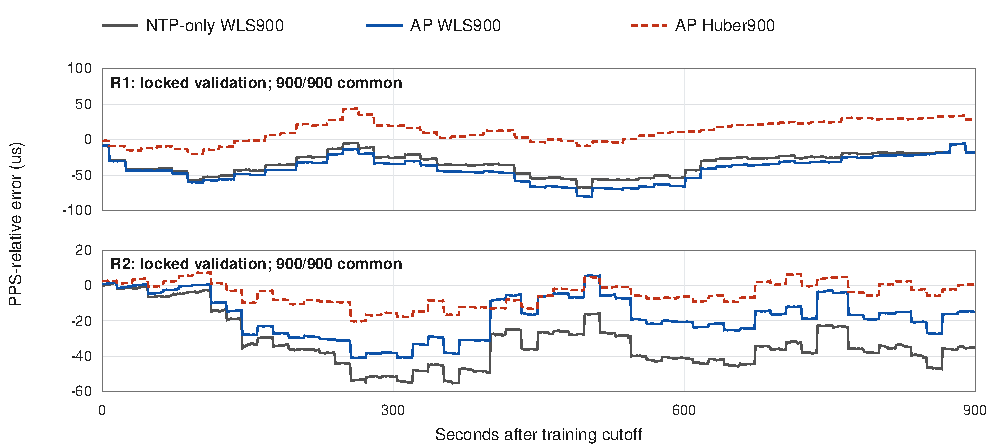
\includegraphics[width=.98\linewidth]{hybrid/phase-curves.pdf}
\caption{SL027 R1--R2 continuously updated affine phase errors: AP-free all-NTP
WLS900, ordinary AP WLS900 and nominated robust AP900, on the same 900 witnesses
per window. Each uses its own prior phase base; parameters are locked before
fresh data. The robust AP's shared-weight local control is in the matrix.
Affine refits can step; phase-continuous servos are not plotted. Vertical scales
differ by panel. No future recentering or rate correction is applied.}
\label{fig:continuous}
\end{figure}
\fi

\subsection{Two fresh locked-validation windows}
Each window retains all 1800 physical PPS, with independently replayed local/AP
maps and NTP anchors. All 13 continuous methods have 900/900 verified future
predictions and prior phase-base histories, with no gaps, mismatches, new fault
increments or bridge resets. R1/R2 retain 97/122 AP and 895/779 local read
refusals without losing these projections. One unpaired pre-window NTP record
remains unknown but enters no retained dependency. Availability is an observed
finite-window result, not a reliability guarantee.

The primary comparison is nominated robust AP900 versus AP-free all-NTP WLS900
(Table~\ref{tab:hybrid-accuracy}, Fig.~\ref{fig:continuous}). Prior-phase-corrected
RMS falls 37.180 to 19.226\us\ in R1 and 35.662 to 8.240\us\ in R2, on the
same 900 future PPS per window. In R1, mean changes from $-34.013$ to
$+11.441\us$, but centered scatter increases from 15.016 to 15.451\us:
the RMS gain is bias reduction, not jitter suppression. R2 reduces both mean
magnitude ($-32.615$ to $-4.790\us$) and scatter (14.425 to 6.704\us).
Its mean-square improvement comprises 86.45\% reduced squared bias and 13.55\%
reduced variance. These are two correlated same-boot windows, not a general
performance distribution.

The complete matrix retains reversals (Table~\ref{tab:hybrid-filters}). Ordinary
AP900 is worse than AP-free WLS900 in R1 (44.904 versus 37.180\us), better in
R2 (21.404 versus 35.662\us). The nominated AP servo60 similarly worsens its
matched local control in R1 but improves it in R2. Shared-Huber local RMS is
24.462/20.397\us; those AP-derived weights make it a secondary mechanism
control, not an AP-free alternative. R2 matched-local WLS900 differs from
all-NTP WLS900 (33.909 versus 35.662\us), exposing input-selection effects as
well. No validation winner replaces either nominee.

Raw phase RMS for AP-free/robust AP is 224.160/217.046\us\ in R1 and
226.778/218.521\us\ in R2. Each method's own 16-PPS prior base produces the
corrected scores; lower corrected RMS does not deliver that accuracy without
external phase calibration. There is no future mean subtraction.

Training accepts 448/449 exchanges in R1/R2, yielding 56 complete burst minima
per run. Native logs count 0/1 discarded training partials; offline candidate
admission counters report 0/0 and remain separate. Both retain 56 training
minima. R2 future admission retains 56 all-NTP versus 55 paired minima, with
one AP-mapping omission. The canonical prior-fit gate rejects none and causes
no reacquisition: real spike-rejection benefit is unproven.
Huber downweighting is a separate positive-weight operation. The observed
all-exchange versus selected-minimum scatter (Table~\ref{tab:hybrid-jitter})
mixes source, path, client and coordinate effects; selection changes its
population and cannot identify isolated source jitter or a fit confidence bound.

Native frozen AP/local forecasts give 35.168/65.843\us\ and
31.777/50.824\us\ RMS across all 900 future PPS
(Table~\ref{tab:hybrid-frozen}). Only 44/58 witnesses have true source age below
60 seconds; their AP RMS is 1.977/2.146\us. Remaining ages extend to 915/901
seconds and represent holdover stress, not continuous service. Post-hoc AP
detrended RMS of 0.936/0.367\us\ characterizes residual precision after removing
future phase/rate; it is not the achieved forecast error or UTC accuracy.

\subsection{Historical comparisons and retained quality failures}
Historical SL025 P1/P2 retain 727/728 common future PPS, respectively, with
172 AP unknowns each and one additional P1 local failure. Their native-known
coordinates, retained/historical inputs and phase bases are independently
checked. Four P2 exchanges with initial history gaps enter no retained target.

P1 AP/local WLS900 gives 19.176/11.234\us\ RMS; shared Huber gives
7.939/10.230\us. In locked P2, AP/local WLS gives 11.529/38.774\us, but robust
AP worsens to 18.889\us. AP/local servo60 changes from 28.987/8.625\us\ in P1
to 10.865/44.146\us\ in P2. Favorable frozen holdover cannot replace these
mixed continuous-service outcomes.

P3 retains 695 native-computed paired opportunities, 204 AP unknowns and one
local failure. Ten native-known AP projections and two retained training
endpoints remain unverified: one needs unrecorded inter-window data; the other
has a short reset epoch unrecognized by the old replay. Unknown fixed-base
dependencies persist after rolling inputs expire. Paired900, Huber and servo
families thus have zero fully verified calibrated P3 errors; only 455 common
short-history errors are fully replayed. All 900 opportunities/native-computed
values remain, without promoting those conditional subsets to replication.

\section{Mechanisms, confounds and earlier failures}
Historical P1 GNSS-relative gains change from $-0.122$ to $+0.474$ ppm local,
but $+7.005$ to $+6.981$ ppm AP. Raw-capture versus mapped-local future gain
differs by only 0.000112 ppm, limiting a bridge-only explanation. These post-hoc
diagnostics never steer a model or locate a physical cause. A frequency-only
1\us\ budget over 60 seconds allows just 0.0167 ppm before other uncertainty.

Validation adds three frozen log rows per PPS. Both methods see the same actual
load, yet logging, interrupts, temperature, supply and uptime may change rate
or software endpoints. Adjacent 60-second parsed-record byte rates increase
9.769\% in R1 and 8.072\% in R2 at freeze; emission-time binning is approximate,
not a CPU/thermal measurement. Zero dropped frames does not establish zero
timing impact; no unique logger/source cause is identified.

The old client also creates availability gaps: resetting AP history after a
failed read requires 32 accepted maps to reacquire; all 172 P1 AP-invalid PPS
lie in that warmup. The P3 queue race retains both raw pulses while refusing
conversion as \texttt{COUNTER\_UNAVAILABLE}. These are client association/history
failures, not missing GNSS/USB records or AP correction telemetry. New firmware
does not retrospectively repair them or explain smooth drift by itself.

Several phase-error hypotheses remain plausible. Starlink server discipline
or software timestamp wander could bias NTP calibration; stratum 1 and zero
reported root fields do not measure source uncertainty. Directional queuing
and software endpoints can change without a large RTT; minimum delay does not
prove reciprocity \citep{nist2016}. Local oscillator/environment variation can
change rate, and small selected samples leave substantial slope leverage
\citep{riley}. One source/path cannot partition those effects. Frozen models
ignore later terminal corrections, whereas continuous targets can inherit
them. AP clock behavior is a separate observation, not terminal correction
telemetry. Smooth AP wander can pass a phase-innovation threshold.

The earlier direct-NTP trials remain a useful negative control. Three clean
SL024 windows retained all 300 future PPS each, with 64.215, 7.795 and
18.737\us\ frozen RMS. The first failure is numerically explained by
$-0.365648$ ppm learned-rate mismatch, accumulating about $-110\us$ in
300 seconds; post-hoc detrending leaves 0.544\us\ RMS without repairing the
forecast. No deterministic timestamp arithmetic bug sufficient to explain that
rate was found. A longer-history model gave 5.424\us\ on one repeat's
\emph{same} witnesses; a 43-PPS short segment at 0.067\us\ was not $67\,\mathrm{ns}$ UTC
accuracy. The earlier incomplete SL023 near-1\us\ record leaves 41 qualified
PPS unreplayed and is context only. Original failures, acquisition attempts and
operator-interrupted populations remain in the evidence history.

\section{Reproduction and qualification limits}
The public supplement retains each future opportunity, qualifier, raw
prediction and own prior base. A standard-library analyzer recomputes errors
and aggregates; it does not recreate acquisition, base-witness measurement or
physical bridge/model publication. Private independent replay checks those
histories and endpoint certificates, binding selected provenance/coverage.
Native frozen models have prospective numeric seals; continuous methods lock
their causal calibration rule before validation. Raw logs, identities,
credentials and images stay private. Paper/figures/derived data are CC BY 4.0;
code/documentation MIT, credited to Jonathan Yantis. Hashes identify bytes,
not accuracy.

The GNSS base absorbs setup/model/path phase bias; it is neither portable nor
a traceable calibration chain \citep{traceability2019}. Receiver/cable/RMC
association, RF-event endpoint, capture/bridge and application mapping remain
uncalibrated. No output edge is measured. Clocks may share dependencies, and
router/terminal hardware/firmware were not inventoried.

Further qualification needs constant logging load, temperature/load records,
reset tests, a calibrated NTP server and independent reference under
counterbalanced conditions. Real source steps require an explicit continuity
policy. Input availability and physical application/output timing need separate
validation.

AP timing is a candidate secondary oscillator, with benefits dependent on
calibration, filtering and coverage. These results do not establish repeatable
microsecond UTC accuracy or a guaranteed horizon. This remains an unapproved
author-review draft, without submission or publication.

\begingroup\small\setlength{\bibsep}{2pt}
\bibliographystyle{unsrtnat}\bibliography{references}\endgroup
\end{document}
